%# -*- coding: utf-8-unix -*-
%%==================================================
%% thesis.tex
%%==================================================

% 双面打印
\documentclass[doctor, fontset=windows, openright, twoside]{sjtuthesis}
% \documentclass[bachelor, fontset=windows, openany, oneside, submit]{sjtuthesis}
% \documentclass[master, fontset=adobe, review]{sjtuthesis}
% \documentclass[%
%   bachelor|master|doctor,	% 必选项
%   fontset=adobe|windows,  	% 只测试了adobe
%   oneside|twoside,		% 单面打印,双面打印(奇偶页交换页边距,默认)
%   openany|openright, 		% 可以在奇数或者偶数页开新章|只在奇数页开新章(默认)
%   zihao=-4|5,, 		% 正文字号:小四、五号(默认)
%   review,	 		% 盲审论文,隐去作者姓名、学号、导师姓名、致谢、发表论文和参与的项目
%   submit			% 定稿提交的论文,插入签名扫描版的原创性声明、授权声明 
% ]

% 逐个导入参考文献数据库
\addbibresource{bib/thesis.bib}
% \addbibresource{bib/chap2.bib}

\begin{document}

%% 无编号内容:中英文论文封面、授权页
%# -*- coding: utf-8-unix -*-
\title{江苏大学学位论文 \LaTeX 模板示例文档}
\author{某\quad{}某}
\advisor{某某教授}
% \coadvisor{某某教授}
\defenddate{2014年12月17日}
\school{江苏大学}
\institute{某某系}
\studentnumber{0010900990}
\major{某某专业}

\englishtitle{A Sample Document for \LaTeX-basedd UJS Thesis Template}
\englishauthor{\textsc{Mo Mo}}
\englishadvisor{Prof. \textsc{Mou Mou}}
% \englishcoadvisor{Prof. \textsc{Uom Uom}}
\englishschool{Jiangsu University}
\englishinstitute{\textsc{Depart of XXX, School of XXX} \\
  \textsc{Jiangsu University} \\
  \textsc{Jiangsu, P.R.China}}
\englishmajor{A Very Important Major}
\englishdate{Dec. 17th, 2014}


\maketitle

\makeenglishtitle

\makeatletter
\ifsjtu@submit\relax
	\includepdf{pdf/original.pdf}
	\cleardoublepage
	\includepdf{pdf/authorization.pdf}
	\cleardoublepage
\else
\ifsjtu@review\relax
% exclude the original claim and authorization
\else
	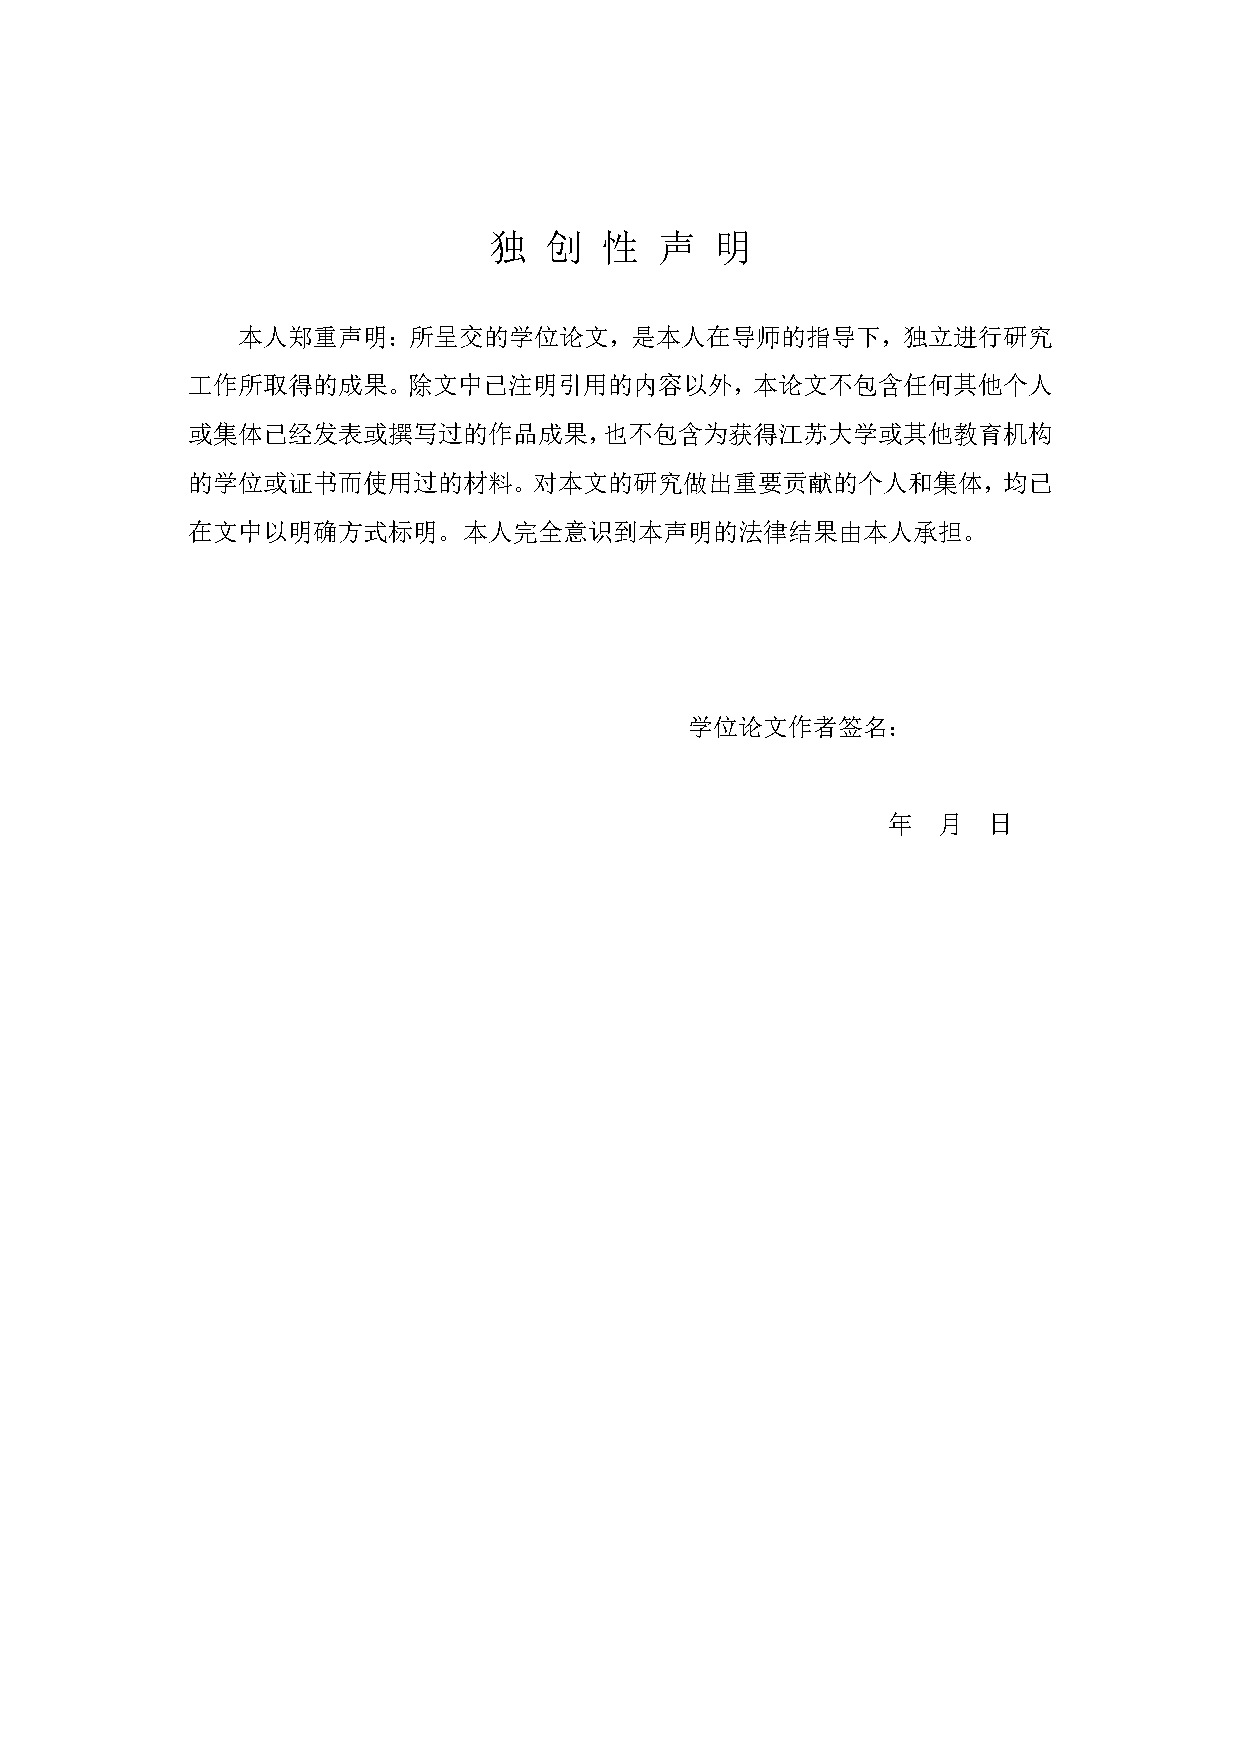
\includepdf{pdf/original_origin.pdf}
	\cleardoublepage
	
\includepdf{pdf/authorization_origin.pdf}
	\cleardoublepage
\fi
\fi
\makeatother


\frontmatter 	% 使用罗马数字对前言编号

%% 摘要
\pagestyle{main}
%# -*- coding: utf-8-unix -*-
%%==================================================
%% abstract.tex for UJS Master Thesis
%%==================================================

\begin{abstract}

江苏大学是2001年8月经教育部批准,由原江苏理工大学、镇江医学院、镇江师范专科学校合并组建。原江苏理工大学的前身镇江农业机械学院,1960年由南京工学院(现东南大学)分设独立建校,1978年被国务院确定为全国88所重点大学之一,1981年成为全国首批具有博士、硕士、学士学位授予权的高校,1982年及1994年先后更名为江苏工学院和江苏理工大学,综合实力一直位居全国高校百强之列。学校坐落在风景秀丽的国家历史文化名城——江苏省镇江市,办学历史可追溯到1902年刘坤一、张之洞等在南京创办的三江师范学堂。 

 学校学科门类齐全,涵盖工学、理学、医学、管理学、经济学、法学、文学、历史学、教育学、艺术学等10大学科门类。设有24个学院,88个本科专业;学校博士学位授权点涵盖13个一级学科,设有13个博士后科研流动站;硕士学位授权点涵盖41个一级学科,有11个硕士专业学位类别,26个工程硕士授权领域。现有2个国家重点学科,1个国家重点(培育)学科,6个江苏高校优势学科。学校的工程学、材料科学、临床医学、化学和农业科学5个学科进入ESI排名全球前1\%(并列全国高校第34位)。2015英国《泰晤士高等教育》第三届金砖国家和新兴经济体大学排名,学校列第181位。中国管理科学研究院《2016中国大学评价》,学校综合排名列全国高校第48位。
 
校园占地面积2822亩,各类建筑面积128余万平方米。教学科研仪器设备总值7.6亿元。图书馆建筑面积5.1万平方米,藏书305余万册,电子图书173余万册,建有教育部科技查新工作站。拥有一所集医疗、教育、科研、预防为一体的三级甲等附属医院。设有江苏大学出版社。

学校现有教职工5763人(含直属附属医院),其中专任教师2475人(教授450余人,具有博士学位的比例达54\%,具有海外经历的比例达24\%),集聚了一批以国家“千人计划”、“长江学者”、国家杰青、国家万人计划领军人才、国家“青年千人计划”为代表的高层次人才群体。在校生33000余人,其中全日制本科生22000余人,研究生10000余人,学历留学生1000余人。江苏大学京江学院全日制在校生近10000人。  
学校是“中央与地方共建高校”、“全国本科教学工作水平优秀高校”、全国“卓越工程师培养计划”首批试点高校、“国家教育体制改革试点高校”、“中国政府奖学金来华留学生接受高校”。近年来,学校获国家级教学成果奖5项,形成了一批以国家特色专业、国家级精品课程、国家精品视频公开课、国家精品资源共享课、国家实验教学示范中心、国家优秀教学团队为代表的优质教学资源;获评“全国百篇优秀博士学位论文”3篇,提名奖5篇;“挑战杯”全国大学生课外学术科技作品竞赛连续5届喜捧“优胜杯”,校大学生男子排球队屡获全国冠军,女子沙滩排球队获世界大学生运动会第7名,女子足球队获世界大学生“五人制”足球锦标赛季军;毕业生就业率一直保持在95\%以上,学校是“全国高校毕业生就业工作先进集体”、“全国50所毕业生就业典型经验高校”和首批“全国高校实践育人创新创业基地”高校和“江苏省大学生创业教育示范学校”。

“十二五”以来,学校科研经费总量达27.89亿元,其中纵向经费8.56亿元;获批国家自然基金项目709项(2014、2015年均居全国高校前50位),其中国家973、863计划等重大重点科技项目52项;获批国家社科基金项目39项;SCI检索收录论文5231篇;截至目前,学校共获得国家级科技成果奖8项、何梁何利基金科学与技术创新奖2项、国家杰出青年基金项目2项;拥有国家水泵及系统工程技术研究中心、混合动力车辆国家地方联合工程中心、国家级新农村发展研究院等3个国家级科技创新平台;建有国家知识产权培训(江苏)基地。学校牵头成立的现代农业装备与技术协同创新中心被认定为江苏省首批高校协同创新中心。2015年度,学校发明专利授权量居全国高校第6位。
学校先后与美国、英国、德国、澳大利亚、奥地利、日本等国家的117所高校及科研机构建立了长期合作关系,与奥地利格拉茨大学共建了孔子学院和汉德语言文化中心。与德国马格德堡大学合作举办了工程热物理专业硕士研究生教育项目,与美国阿卡迪亚大学合作开办了数学与应用数学专业本科教育项目。
学校坚持以人为本,大力推进和谐校园、民主法治和校园文化建设,党建创新不断加强。学校党委被中央组织部表彰为全国创先争优先进基层党组织,连续两次被评为江苏省“高校先进基层党组织”。学校多次获江苏省文明单位、和谐校园、平安校园等荣誉称号。

目前,江苏大学正高举中国特色社会主义伟大旗帜,深入贯彻党的十八大和习近平总书记系列重要讲话精神,紧紧围绕学校第三次党代会确定的奋斗目标,汇聚全校师生的智慧和力量,坚定不移地走以提升质量、强化特色为核心的内涵式发展道路,为把学校早日建成“高水平、有特色、国际化研究型大学”而努力奋斗!

\keywords{\large 江苏大学 \quad 博学 \quad 求是 \quad 明德}
\end{abstract}

\begin{englishabstract}

Jiangsu University (JSU) was founded in 1902 as a part of Sanjiang Normal University. It was retitled as Jiangsu University by integrating Jiangsu University of Science and Technology, Zhenjiang Medical College and Zhenjiang Teachers’ College with the approval of the Ministry of Education of China in August, 2001. The university’s undergraduate teaching was graded excellent by the Ministry of Education in 2004. It has developed to be a national comprehensive key university. According to the Evaluations of China’s Universities in 2017 by China Academy of Management Science, JSU is ranked 41. It is committed to cultivating talents with 4C (Confidence, Communication, Cooperation and Creation). Now the university is launching the new orientation of schooling for high-level, research-oriented university with strength of engineering and strategy of internationalization.
 
JSU offers 88 undergraduate programs, 170 master programs, and 42 PhD programs in 10 academic fields: Engineering, Science, Management, Economics, Medicine, Law, Education, Literature, Art and History. The university has 13 post-doctoral research stations. Distinguished among its peers for its academic rigor, the 24 schools are competing and collaborating with each other for a high-level, research-oriented university with distinctive features and internationalization strategy.

JSU has 5,763 staff members (including those of Affiliated Hospital). 2,475 are faculty members, including 450 professors. 54\% of them have got Ph.D degrees and over 24\% have experience of overseas study. The current total enrollment of full-time students amounts to over 33,000, including 10,000 postgraduates, 1000 international students from 74 countries. Jingjiang College of Jiangsu Univesity has an enrollement of about 10000 full-time students.

JSU has been promoting high-level research. In the recent 5 years, the total scientific research fund amounts to 2.789 billion RMB, sponsored by the governments and enterprises. The number of authorized is ranked 6 among China’s universities. Five disciplines have been ranked as top 1\% in ESI, such as Engineering, Clinical Medicine, Materials Science, Chemistry and Agricultural Science. Drawing on the big varieties of programs and multi-disciplinary strengths, we operate an array of research institutes and centers serving as both the academic think tanks and technological innovation source at the national and regional levels. 

JSU gives priorities to the internationalization of the schooling, encouraging faculty members and students to go abroad for further studies, inviting more global talents to join us for mutual benefits, promoting international research collaboration as well as recruiting more overseas students.

JSU has signed institutional cooperation agreements with 128 universities in 33 countries and regions by May 2017. The Confucius Institute co-built by JSU and Graz University (Austria) has been operating smoothly since October 2010, followed by the opening of the collaborative Chinese-German Language and Culture Center.

\englishkeywords{\large UJS, master thesis, XeTeX/LaTeX template}
\end{englishabstract}



%% 目录、插图目录、表格目录
\tableofcontents
\listoffigures
\addcontentsline{toc}{chapter}{\listfigurename} %将插图目录加入全文目录
\listoftables
\addcontentsline{toc}{chapter}{\listtablename}  %将表格目录加入全文目录
\listofalgorithms
\addcontentsline{toc}{chapter}{算法索引}        %将算法目录加入全文目录

\include{tex/symbol} % 主要符号、缩略词对照表

\mainmatter	% 使用阿拉伯数字对正文编号

%% 正文内容
\pagestyle{main}
%# -*- coding: utf-8-unix -*-
%%==================================================
%% chapter01.tex for SJTU Master Thesis
%%==================================================

%\bibliographystyle{sjtu2}%[此处用于每章都生产参考文献]
\chapter{这是什么}
\label{chap:intro}

这是江苏大学(非官方)学位论文 \LaTeX 模板,是基于于 GitHub 上海交通大学版本为 \version 的 \LaTeX 模板上修改而成。

最早的一版学位模板是一位热心的物理系同学制作的。
那份模板参考了自动化所学位论文模板,使用了CASthesis.cls文档类,中文字符处理则采用当时最为流行的 \CJKLaTeX 方案。
我根据交大研究生院对学位论文的要求
\footnote{\url{http://www.gs.sjtu.edu.cn/policy/fileShow.ahtml?id=130}}
,结合少量个人审美喜好,完成了一份基本可用的交大 \LaTeX 学位论文模板。
但是,搭建一个 \CJKLaTeX 环境并不简单,单单在Linux下配置环境和添加中文字体,就足够让新手打退堂鼓。
在William Wang的建议下,我开始着手把模板向 \XeTeX 引擎移植。
他完成了最初的移植,多亏了他出色的工作,后续的改善工作也得以顺利进行。

随着我对 \LaTeX 系统认知增加,我又断断续续做了一些完善模板的工作,在原有硕士学位论文模板的基础上完成了交大学士和博士学位论文模板。

现在,交大学位论文模板SJTUTHesis代码在github
\footnote{\url{https://github.com/weijianwen/SJTUThesis}}
上维护。
你可以\href{https://github.com/weijianwen/SJTUThesis/issues}{在github上开issue}
、或者在\href{https://bbs.sjtu.edu.cn/bbsdoc?board=TeX_LaTeX}{水源LaTeX版}发帖来反映遇到的问题。

\section{使用模板}

\subsection{准备工作}
\label{sec:requirements}

要使用这个模板撰写学位论文,需要在\emph{TeX系统}、\emph{中英文字体}、\emph{TeX技能}上有所准备。

\begin{itemize}[noitemsep,topsep=0pt,parsep=0pt,partopsep=0pt]
	\item {\TeX}系统:所使用的{\TeX}系统要支持 \XeTeX 引擎,且带有ctex 2.x宏包,以2015年的\emph{完整}TeXLive、MacTeX发行版为佳。
	\item 中英文字体:操作系统中需要安装\footnote{在Windows、Mac OS X 以及 Linux 上安装额外的字体,可以参考\href{https://www.searchfreefonts.com/articles/how-to-install-fonts.htm}{“How to install fonts?”}。
}TeX Gyre Termes字体\footnote{\url{http://www.gust.org.pl/projects/e-foundry/tex-gyre/termes}}和四款Adobe中文字体
\footnote{请从合法渠道获得Adobe字体。}:AdobeSongStd、AdobeKaitiStd、AdobeHeitiStd、AdobeFangsongStd。
	\item TeX技能:尽管提供了对模板的必要说明,但这不是一份“ \LaTeX 入门文档”。在使用前请先通读其他入门文档。
	\item 针对Windows用户的额外需求:学位论文模本分别使用git和GNUMake进行版本控制和构建,建议从Cygwin\footnote{\url{http://cygwin.com}}安装这两个工具。
\end{itemize}

\subsection{模板选项}
\label{sec:thesisoption}

sjtuthesis提供了一些常用选项,在thesis.tex在导入sjtuthesis模板类时,可以组合使用。
这些选项包括:

\begin{itemize}[noitemsep,topsep=0pt,parsep=0pt,partopsep=0pt]
\item 学位类型:bachelor(学位)、master(硕士)、doctor(博士),是必选项。
\item 中国字体:adobefonts(Adobe中文字体)、winfonts(使用Windows下的中文字体,该选项未在Linux/Mac下测试)。
\item 正文字号:cs4size(小四)、c5size(五号)。
\item 盲审选项:使用review选项后,论文作者、学号、导师姓名、致谢、发表论文和参与项目将被隐去。
\end{itemize}

\subsection{编译模板}
\label{sec:process}

模板默认使用GNUMake构建,GNUMake将调用latemk工具自动完成模板多轮编译:

\begin{lstlisting}[basicstyle=\small\ttfamily, caption={编译模板}, numbers=none]
make clean thesis.pdf
\end{lstlisting}

若需要生成包含“原创性声明扫描件”的学位论文文档,请将扫描件保存为statement.pdf,然后调用make生成submit.pdf。

\begin{lstlisting}[basicstyle=\small\ttfamily, caption={生成用于提交的学位论文}, numbers=none]
make clean submit.pdf
\end{lstlisting}

编译失败时,可以尝试手动逐次编译,定位故障。

\begin{lstlisting}[basicstyle=\small\ttfamily, caption={手动逐次编译}, numbers=none]
xelatex -no-pdf thesis
biber --debug thesis
xelatex thesis
xelatex thesis
\end{lstlisting}

\subsection{模板文件布局}
\label{sec:layout}

\begin{lstlisting}[basicstyle=\small\ttfamily,caption={模板文件布局},label=layout,float,numbers=none]
├── LICENSE
├── Makefile
├── README.md
├── bib
│   ├── chap1.bib
│   └── chap2.bib
├── bst
│   └── GBT7714-2005NLang.bst
├── figure
│   ├── chap2
│   │   ├── sjtulogo.eps
│   │   ├── sjtulogo.jpg
│   │   ├── sjtulogo.pdf
│   │   └── sjtulogo.png
│   └── sjtubanner.png
├── sjtuthesis.cfg
├── sjtuthesis.cls
├── statement.pdf
├── submit.pdf
├── tex
│   ├── abstract.tex
│   ├── ack.tex
│   ├── app_cjk.tex
│   ├── app_eq.tex
│   ├── app_log.tex
│   ├── chapter01.tex
│   ├── chapter02.tex
│   ├── chapter03.tex
│   ├── conclusion.tex
│   ├── id.tex
│   ├── patents.tex
│   ├── projects.tex
│   ├── pub.tex
│   └── symbol.tex
└── thesis.tex
\end{lstlisting}

本节介绍学位论文模板中木要文件和目录的功能。

\subsubsection{格式控制文件}
\label{sec:format}

格式控制文件控制着论文的表现形式,包括以下几个文件:
sjtuthesis.cfg, sjtuthesis.cls和GBT7714-2005NLang.bst。
其中,“cfg”和“cls”控制论文主体格式,“bst”控制参考文献条目的格式,

\subsubsection{主控文件thesis.tex}
\label{sec:thesistex}

主控文件thesis.tex的作用就是将你分散在多个文件中的内容“整合”成一篇完整的论文。
使用这个模板撰写学位论文时,你的学位论文内容和素材会被“拆散”到各个文件中:
譬如各章正文、各个附录、各章参考文献等等。
在thesis.tex中通过“include”命令将论文的各个部分包含进来,从而形成一篇结构完成的论文。
对模板定制时引入的宏包,建议放在导言区。

\subsubsection{各章源文件tex}
\label{sec:thesisbody}

这一部分是论文的主体,是以“章”为单位划分的,包括:

\begin{itemize}[noitemsep,topsep=0pt,parsep=0pt,partopsep=0pt]
	\item 中英文摘要(abstract.tex)。前言(frontmatter)的其他部分,中英文封面、原创性声明、授权信息在sjtuthesis.cls中定义,不单独分离为tex文件。
不单独弄成文件。
	\item 正文(mainmatter)——学位论文正文的各章内容,源文件是chapter\emph{xxx}.tex。
	\item 附录(app\emph{xx}.tex)、致谢(thuanks.tex)、攻读学位论文期间发表的学术论文目录(pub.tex)、个人简历(resume.tex)组成正文后的部分(backmatter)。
参考文献列表由bibtex插入,不作为一个单独的文件。
\end{itemize}

\subsubsection{图片文件夹figure}
\label{sec:fig}

figure文件夹放置了需要插入文档中的图片文件(支持PNG/JPG/PDF/EPS格式的图片),可以在按照章节划分子目录。
模板文件中使用\verb|\graphicspath|命令定义了图片存储的顶层目录,在插入图片时,顶层目录名“figure”可省略。

\subsubsection{参考文献数据库bib}
\label{sec:bib}

目前参考文件数据库目录只存放一个参考文件数据库thesis.bib。
关于参考文献引用,可参考第\ref{chap:example}章中的例子。


%# -*- coding: utf-8-unix -*-
%%==================================================
%% chapter02.tex for UJS Master Thesis
%% based on CASthesis
%% modified by wei.jianwen@gmail.com
%% Encoding: UTF-8
%%==================================================

\chapter{ \LaTeX 排版例子}
\label{chap:example}

\section{列表环境}
\label{sec:list}

\subsection{无序列表}
\label{sec:unorderlist}

以下是一个无序列表的例子,列表的每个条目单独分段。

\begin{itemize}
  \item 这是一个无序列表。
  \item 这是一个无序列表。
  \item 这是一个无序列表。
\end{itemize}

使用\verb+itemize*+环境可以创建行内无序列表。
\begin{itemize*}
  \item 这是一个无序列表。
  \item 这是一个无序列表。
  \item 这是一个无序列表。
\end{itemize*}
行内无序列表条目不单独分段,所有内容直接插入在原文的段落中。

\subsection{有序列表}
\label{sec:orderlist}

使用环境\verb+enumerate+和\verb+enumerate*+创建有序列表,
使用方法无序列表类似。

\begin{enumerate}
  \item 这是一个有序列表。
  \item 这是一个有序列表。
  \item 这是一个有序列表。
\end{enumerate}

使用\verb+enumerate*+环境可以创建行内有序列表。
\begin{enumerate*}
  \item 这是一个默认有序列表。
  \item 这是一个默认有序列表。
  \item 这是一个默认有序列表。
\end{enumerate*}
行内有序列表条目不单独分段,所有内容直接插入在原文的段落中。

\subsection{描述型列表}

使用环境\verb+description+可创建带有主题词的列表,条目语法是\verb+\item[主题] 内容+。
\begin{description}
    \item[主题一] 详细内容
    \item[主题二] 详细内容
    \item[主题三] 详细内容 \ldots
\end{description}

\subsection{自定义列表样式}

可以使用\verb+label+参数控制列表的样式,
详细可以参考WikiBooks\footnote{\url{https://en.wikibooks.org/wiki/LaTeX/List_Structures\#Customizing_lists}}。
比如一个自定义样式的行内有序列表
\begin{enumerate*}[label=\itshape\alph*)\upshape]
  \item 这是一个自定义样式有序列表。
  \item 这是一个自定义样式有序列表。
  \item 这是一个自定义样式有序列表。
\end{enumerate*}

\section{数学排版}
\label{sec:matheq}

\subsection{公式排版}
\label{sec:eqformat}

这里有举一个长公式排版的例子,来自\href{http://www.tex.ac.uk/tex-archive/info/math/voss/mathmode/Mathmode.pdf}{《Math mode》}:

\begin {multline}
  \frac {1}{2}\Delta (f_{ij}f^{ij})=
  2\left (\sum _{i<j}\chi _{ij}(\sigma _{i}-
    \sigma _{j}) ^{2}+ f^{ij}\nabla _{j}\nabla _{i}(\Delta f)+\right .\\
  \left .+\nabla _{k}f_{ij}\nabla ^{k}f^{ij}+
    f^{ij}f^{k}\left [2\nabla _{i}R_{jk}-
      \nabla _{k}R_{ij}\right ]\vphantom {\sum _{i<j}}\right )
\end{multline}

\subsection{SI单位}

使用\verb+siunitx+宏包可以方便地输入SI单位制单位,例如\verb+\SI{5}{\um}+可以得到\SI{5}{\um}。

\subsubsection{一个四级标题}
\label{sec:depth4}

这是全文唯一的一个四级标题。在这部分中将演示了mathtools宏包中可伸长符号(箭头、等号的例子)的例子。

\begin{displaymath}
    A \xleftarrow[n=0]{} B \xrightarrow[LongLongLongLong]{n>0} C 
\end{displaymath}

\begin{eqnarray}
  f(x) & \xleftrightarrow[]{A=B}  & B \\
  & \xleftharpoondown[below]{above} & B \nonumber \\
  & \xLeftrightarrow[below]{above} & B
\end{eqnarray}

又如:

\begin{align}
  \label{eq:none}
  & I(X_3;X_4)-I(X_3;X_4\mid{}X_1)-I(X_3;X_4\mid{}X_2) \nonumber \\
  = & [I(X_3;X_4)-I(X_3;X_4\mid{}X_1)]-I(X_3;X_4\mid{}\tilde{X}_2) \\
  = & I(X_1;X_3;X_4)-I(X_3;X_4\mid{}\tilde{X}_2)
\end{align}

\subsection{定理环境}

模板中定义了丰富的定理环境
algo(算法),thm(定理),lem(引理),prop(命题),cor(推论),defn(定义),conj(猜想),exmp(例),rem(注),case(情形),
bthm(断言定理),blem(断言引理),bprop(断言命题),bcor(断言推论)。
amsmath还提供了一个proof(证明)的环境。
这里举一个“定理”和“证明”的例子。
\begin{thm}[留数定理]
\label{thm:res}
  假设$U$是复平面上的一个单连通开子集,$a_1,\ldots,a_n$是复平面上有限个点,$f$是定义在$U\backslash \{a_1,\ldots,a_n\}$上的全纯函数,
  如果$\gamma$是一条把$a_1,\ldots,a_n$包围起来的可求长曲线,但不经过任何一个$a_k$,并且其起点与终点重合,那么:

  \begin{equation}
    \label{eq:res}
    \ointop_{\gamma}f(z)\,\mathrm{d}z = 2\uppi\mathbf{i}\sum^n_{k=1}\mathrm{I}(\gamma,a_k)\mathrm{Res}(f,a_k)
  \end{equation}

  如果$\gamma$是若尔当曲线,那么$\mathrm{I}(\gamma, a_k)=1$,因此:

  \begin{equation}
    \label{eq:resthm}
    \ointop_{\gamma}f(z)\,\mathrm{d}z = 2\uppi\mathbf{i}\sum^n_{k=1}\mathrm{Res}(f,a_k)
  \end{equation}

      % \oint_\gamma f(z)\, dz = 2\pi i \sum_{k=1}^n \mathrm{Res}(f, a_k ). 

  在这里,$\mathrm{Res}(f, a_k)$表示$f$在点$a_k$的留数,$\mathrm{I}(\gamma,a_k)$表示$\gamma$关于点$a_k$的卷绕数。
  卷绕数是一个整数,它描述了曲线$\gamma$绕过点$a_k$的次数。如果$\gamma$依逆时针方向绕着$a_k$移动,卷绕数就是一个正数,
  如果$\gamma$根本不绕过$a_k$,卷绕数就是零。

  定理\ref{thm:res}的证明。
  
  \begin{proof}
    首先,由……

    其次,……

    所以……
  \end{proof}
\end{thm}

上面的公式例子中,有一些细节希望大家注意。微分号d应该使用“直立体”也就是用mathrm包围起来。
并且,微分号和被积函数之间应该有一段小间隔,可以插入\verb+\,+得到。
斜体的$d$通常只作为一般变量。
i,j作为虚数单位时,也应该使用“直立体”为了明显,还加上了粗体,例如\verb+\mathbf{i}+。斜体$i,j$通常用作表示“序号”。
其他字母在表示常量时,也推荐使用“直立体”譬如,圆周率$\uppi$(需要upgreek宏包),自然对数的底$\mathrm{e}$。
不过,我个人觉得斜体的$e$和$\pi$很潇洒,在不至于引起混淆的情况下,我也用这两个字母的斜体表示对应的常量。


\section{向文档中插入图像}
\label{sec:insertimage}

\subsection{支持的图片格式}
\label{sec:imageformat}

\XeTeX 可以很方便地插入PDF、PNG、JPG格式的图片。

插入PNG/JPG的例子如\ref{fig:SRR}所示。
这两个水平并列放置的图共享一个“图标题”(table caption),没有各自的小标题。

\begin{figure}[!htp]
  \centering
  \includegraphics[width=0.3\textwidth]{example/sjtulogo.png}
  \hspace{1cm}
  \includegraphics[width=0.3\textwidth]{example/sjtulogo.jpg}
  \bicaption[fig:SRR]{这里将出现在插图索引中}{中文题图}{Fig}{English caption}
\end{figure}

% 这里还有插入eps图像和pdf图像的例子,如图\ref{fig:epspdf:a}和图\ref{fig:epspdf:b}。这里将EPS和PDF图片作为子图插入,每个子图有自己的小标题。并列子图的功能是使用subfigure宏包提供的。
% 
% \begin{figure}
%   \centering
%   \subfigure[EPS Figure]{
%     \label{fig:epspdf:a} %% label for first subfigure
%     \includegraphics[width=0.3\textwidth]{example/sjtulogo.eps}}
%   \hspace{1in}
%   \subfigure[PDF Figure]{
%     \label{fig:epspdf:b} %% label for second subfigure
%     \includegraphics[width=0.3\textwidth]{example/sjtulogo.pdf}}
%   \bicaption[fig:pdfeps]{插入eps图像和pdf图像}{插入eps和pdf的例子}{Fig}{An EPS and PDF demo}
% \end{figure}

更多关于 \LaTeX 插图的例子可以参考\href{http://www.cs.duke.edu/junhu/Graphics3.pdf}{《\LaTeX 插图指南》}。

\subsection{长标题的换行}
\label{sec:longcaption}

图\ref{fig:longcaptionbad}和图\ref{fig:longcaptiongood}都有比较长图标题,通过对比发现,图\ref{fig:longcaptiongood}的换行效果更好一些。
其中使用了minipage环境来限制整个浮动体的宽度。

\begin{figure}[!htp]
 \centering
 \includegraphics[width=4cm]{example/sjtulogo.pdf}
 \bicaption[fig:longcaptionbad]{这里将出现在插图索引}{海交通大学是我国历史最悠久的高等学府之一,是教育部直属、教育部与上海市共建的全国重点大学.}{Fig}{Where there is a will, there is a way.}
\end{figure}

\begin{figure}[!htbp]
  \centering
  \begin{minipage}[b]{0.6\textwidth}
    \captionstyle{\centering}
    \centering
    \includegraphics[width=4cm]{example/sjtulogo.pdf}
    \bicaption[fig:longcaptiongood]{这里将出现在插图索引}{海交通大学是我国历史最悠久的高等学府之一,是教育部直属、教育部与上海市共建的全国重点大学.}{Fig}{Where there is a will, there is a way.}
  \end{minipage}     
\end{figure}

\subsection{绘制流程图}

图\ref{fig:flow_chart}是一张流程图示意。使用tikz环境,搭配四种预定义节点(\verb+startstop+、\verb+process+、\verb+decision+和\verb+io+),可以容易地绘制出流程图。
\begin{figure}[!htp]
    \centering
    \resizebox{6cm}{!}{\input{figure/example/flow_chart.tex}}
    \bicaption[fig:flow_chart]{绘制流程图效果}{流程图}{Fig}{Flow chart}
\end{figure}
  
\clearpage

\section{表格}
\label{sec:tab}

这一节给出的是一些表格的例子,如表\ref{tab:firstone}所示。

\begin{table}[!hpb]
  \centering
  \bicaption[tab:firstone]{指向一个表格的表目录索引}{一个颇为标准的三线表格\footnotemark[1]}{Table}{A Table}
  \begin{tabular}{@{}llr@{}} \toprule
    \multicolumn{2}{c}{Item} \\ \cmidrule(r){1-2}
    Animal & Description & Price (\$)\\ \midrule
    Gnat & per gram & 13.65 \\
    & each & 0.01 \\
    Gnu & stuffed & 92.50 \\
    Emu & stuffed & 33.33 \\
    Armadillo & frozen & 8.99 \\ \bottomrule
  \end{tabular}
\end{table}
\footnotetext[1]{这个例子来自\href{http://www.ctan.org/tex-archive/macros/latex/contrib/booktabs/booktabs.pdf}{《Publication quality tables in LATEX》}(booktabs宏包的文档)。这也是一个在表格中使用脚注的例子,请留意与threeparttable实现的效果有何不同。}

下面一个是一个更复杂的表格,用threeparttable实现带有脚注的表格,如表\ref{tab:footnote}。

\begin{table}[!htpb]
  \bicaption[tab:footnote]{出现在表目录的标题}{一个带有脚注的表格的例子}{Table}{A Table with footnotes}
  \centering
  \begin{threeparttable}[b]
     \begin{tabular}{ccd{4}cccc}
      \toprule
      \multirow{2}{6mm}{total}&\multicolumn{2}{c}{20\tnote{1}} & \multicolumn{2}{c}{40} &  \multicolumn{2}{c}{60}\\
      \cmidrule(lr){2-3}\cmidrule(lr){4-5}\cmidrule(lr){6-7}
      &www & k & www & k & www & k \\
      \midrule
      &$\underset{(2.12)}{4.22}$ & 120.0140\tnote{2} & 333.15 & 0.0411 & 444.99 & 0.1387 \\
      &168.6123 & 10.86 & 255.37 & 0.0353 & 376.14 & 0.1058 \\
      &6.761    & 0.007 & 235.37 & 0.0267 & 348.66 & 0.1010 \\
      \bottomrule
    \end{tabular}
    \begin{tablenotes}
    \item [1] the first note.% or \item [a]
    \item [2] the second note.% or \item [b]
    \end{tablenotes}
  \end{threeparttable}
\end{table}

\section{参考文献管理}

 \LaTeX 具有将参考文献内容和表现形式分开管理的能力,涉及三个要素:参考文献数据库、参考文献引用格式、在正文中引用参考文献。
这样的流程需要多次编译:

\begin{enumerate}[noitemsep,topsep=0pt,parsep=0pt,partopsep=0pt]
	\item 用户将论文中需要引用的参考文献条目,录入纯文本数据库文件(bib文件)。
	\item 调用xelatex对论文模板做第一次编译,扫描文中引用的参考文献,生成参考文献入口文件(aux)文件。
	\item 调用bibtex,以参考文献格式和入口文件为输入,生成格式化以后的参考文献条目文件(bib)。
	\item 再次调用xelatex编译模板,将格式化以后的参考文献条目插入正文。
\end{enumerate}

参考文献数据库(thesis.bib)的条目,可以从Google Scholar搜索引擎\footnote{\url{https://scholar.google.com}}、CiteSeerX搜索引擎\footnote{\url{http://citeseerx.ist.psu.edu}}中查找,文献管理软件Papers\footnote{\url{http://papersapp.com}}、Mendeley\footnote{\url{http://www.mendeley.com}}、JabRef\footnote{\url{http://jabref.sourceforge.net}}也能够输出条目信息。

下面是在Google Scholar上搜索到的一条文献信息,格式是纯文本:

\begin{lstlisting}[caption={从Google Scholar找到的参考文献条目}, label=googlescholar, escapeinside="", numbers=none]
    @phdthesis{"白2008信用风险传染模型和信用衍生品的定价",
      title={"信用风险传染模型和信用衍生品的定价"},
      author={"白云芬"},
      year={2008},
      school={"上海交通大学"}
    } 
\end{lstlisting}

推荐修改后在bib文件中的内容为:

\begin{lstlisting}[caption={修改后的参考文献条目}, label=itemok, escapeinside="", numbers=none]
  @phdthesis{bai2008,
    title={"信用风险传染模型和信用衍生品的定价"},
    author={"白云芬"},
    date={2008},
    address={"上海"},
    school={"上海交通大学"}
  } 
\end{lstlisting}

按照教务处的要求,参考文献外观应符合国标GBT7714的要求\footnote{\url{http://www.cces.net.cn/guild/sites/tmxb/Files/19798_2.pdf}}。
在模板中,表现形式的控制逻辑通过bibla­tex-gb7714-2015包实现\footnote{\url{https://www.ctan.org/pkg/biblatex-gb7714-2015}},基于{Bib\LaTeX}管理文献。在目前的多数TeX发行版中,可能都没有默认包含biblatex-gb7714-2015,需要手动安装。

正文中引用参考文献时,用\verb+\cite{key1,key2,key3...}+可以产生“上标引用的参考文献”,
如\cite{Meta_CN,chen2007act,DPMG}。
使用\verb+\citen{key1,key2,key3...}+则可以产生水平引用的参考文献,例如\citen{JohnD,zhubajie,IEEE-1363}。
请看下面的例子,将会穿插使用水平的和上标的参考文献:关于书的\citen{Meta_CN,JohnD,IEEE-1363},关于期刊的\cite{chen2007act,chen2007ewi},
会议论文\citen{DPMG,kocher99,cnproceed},
硕士学位论文\citen{zhubajie,metamori2004},博士学位论文\cite{shaheshang,FistSystem01,bai2008},标准文件\citen{IEEE-1363},技术报告\cite{NPB2},电子文献\citen{xiaoyu2001, CHRISTINE1998},用户手册\citen{RManual}。

总结一些注意事项:
\begin{itemize}
\item 参考文献只有在正文中被引用了,才会在最后的参考文献列表中出现;
\item 参考文献“数据库文件”bib是纯文本文件,请使用UTF-8编码,不要使用GBK编码;
\item 参考文献条目中默认通过date域输入时间。兼容使用year域时会产生编译warning,可忽略。
\end{itemize}

\section{用listings插入源代码}

原先ctexbook文档类和listings宏包配合使用时,代码在换页时会出现莫名其妙的错误,后来经高人指点,顺利解决了。
感兴趣的话,可以看看\href{http://bbs.ctex.org/viewthread.php?tid=53451}{这里}。
这里给使用listings宏包插入源代码的例子,这里是一段C代码。
另外,listings宏包真可谓博大精深,可以实现各种复杂、漂亮的效果,想要进一步学习的同学,可以参考
\href{http://mirror.ctan.org/macros/latex/contrib/listings/listings.pdf}{listings宏包手册}。

\begin{lstlisting}[language={C}, caption={一段C源代码}]
#include <stdio.h>
#include <unistd.h>
#include <sys/types.h>
#include <sys/wait.h>

int main() {
  pid_t pid;

  switch ((pid = fork())) {
  case -1:
    printf("fork failed\n");
    break;
  case 0:
    /* child calls exec */
    execl("/bin/ls", "ls", "-l", (char*)0);
    printf("execl failed\n");
    break;
  default:
    /* parent uses wait to suspend execution until child finishes */
    wait((int*)0);
    printf("is completed\n");
    break;
  }

  return 0;
}
\end{lstlisting}

\section{用algorithm和algorithmicx宏包插入算法描述}

algorithmicx 比 algorithmic 增加了一些命令。
示例如算法\ref{algo:sum_100}和算法\ref{algo:merge_sort},
后者的代码来自\href{http://hustsxh.is-programmer.com/posts/38801.html}{xhSong的博客}。
algorithmicx的详细使用方法见\href{http://mirror.hust.edu.cn/CTAN/macros/latex/contrib/algorithmicx/algorithmicx.pdf}{官方README}。
使用算法宏包时,算法出现的位置很多时候不按照tex文件里的书写顺序, 
需要强制定位时可以使用\verb+\begin{algorithm}[H]+
\footnote{http://tex.stackexchange.com/questions/165021/fixing-the-location-of-the-appearance-in-algorithmicx-environment}

这是写在算法\ref{algo:sum_100}前面的一段话,在生成的文件里它会出现在算法\ref{algo:sum_100}前面。

\begin{algorithm}
% \begin{algorithm}[H] % 强制定位
\caption{求100以内的整数和}
\label{algo:sum_100}
\begin{algorithmic}[1] %每行显示行号
\Ensure 100以内的整数和 % 输出
\State $sum \gets 0$
\For{$i = 0 \to 100$}
    \State $sum \gets sum + i$
  \EndFor
\end{algorithmic}
\end{algorithm}

这是写在两个算法中间的一段话,当算法\ref{algo:sum_100}不使用\verb+\begin{algorithm}[H]+时它也会出现在算法\ref{algo:sum_100}前面。

对于很长的算法,单一的算法块\verb+\begin{algorithm}...\end{algorithm}+是不能自动跨页的
\footnote{http://tex.stackexchange.com/questions/70733/latex-algorithm-not-display-under-correct-section},
会出现的情况有:

\begin{itemize}
  \item 该页放不下当前的算法,留下大片空白,算法在下一页显示
  \item 单一页面放不下当前的算法,显示时超过页码的位置直到超出整个页面范围
\end{itemize}

解决方法有:

\begin{itemize}
  \item (推荐)使用\verb+algstore{algname}+和\verb+algrestore{algname}+来讲算法分为两个部分\footnote{http://tex.stackexchange.com/questions/29816/algorithm-over-2-pages},如算法\ref{algo:merge_sort}。
  \item 人工拆分算法为多个小的部分。
\end{itemize}

\begin{algorithm}
% \begin{algorithm}[H] % 强制定位
\caption{用归并排序求逆序数}
\label{algo:merge_sort}
\begin{algorithmic}[1] %每行显示行号
\Require $Array$数组,$n$数组大小 % 输入
\Ensure 逆序数 % 输出
\Function {MergerSort}{$Array, left, right$}
  \State $result \gets 0$
  \If {$left < right$}
    \State $middle \gets (left + right) / 2$
    \State $result \gets result +$ \Call{MergerSort}{$Array, left, middle$}
    \State $result \gets result +$ \Call{MergerSort}{$Array, middle, right$}
    \State $result \gets result +$ \Call{Merger}{$Array,left,middle,right$}
  \EndIf
  \State \Return{$result$}
\EndFunction
\State %空一行
\Function{Merger}{$Array, left, middle, right$}
  \State $i\gets left$
  \State $j\gets middle$
  \State $k\gets 0$
  \State $result \gets 0$
  \While{$i<middle$ \textbf{and} $j<right$}
    \If{$Array[i]<Array[j]$}
      \State $B[k++]\gets Array[i++]$
    \Else
      \State $B[k++] \gets Array[j++]$
      \State $result \gets result + (middle - i)$
    \EndIf
  \EndWhile
  \algstore{MergeSort}
\end{algorithmic}
\end{algorithm}

\begin{algorithm}
\begin{algorithmic}[1]
  \algrestore{MergeSort}
  \While{$i<middle$}
    \State $B[k++] \gets Array[i++]$
  \EndWhile
  \While{$j<right$}
    \State $B[k++] \gets Array[j++]$
  \EndWhile
  \For{$i = 0 \to k-1$}
    \State $Array[left + i] \gets B[i]$
  \EndFor
  \State \Return{$result$}
\EndFunction
\end{algorithmic}
\end{algorithm}

这是写在算法\ref{algo:merge_sort}后面的一段话,
但是当算法\ref{algo:merge_sort}不使用\verb+\begin{algorithm}[H]+时它会出现在算法\ref{algo:merge_sort}
甚至算法\ref{algo:sum_100}前面。

对于算法的索引要注意\verb+\caption+和\verb+\label+的位置, 
必须是先\verb+\caption+再\verb+\label+\footnote{http://tex.stackexchange.com/questions/65993/algorithm-numbering},
否则会出现\verb+\ref{algo:sum_100}+生成的编号跟对应算法上显示不一致的问题。

根据Werner的回答\footnote{http://tex.stackexchange.com/questions/53357/switch-cases-in-algorithmic}
增加了\verb+Switch+和\verb+Case+的支持,见算法\ref{algo:switch_example}。

\begin{algorithm}
\caption{Switch示例}
\label{algo:switch_example}
\begin{algorithmic}[1]
  \Switch{$s$}
    \Case{$a$}
      \Assert{0}
    \EndCase
    \Case{$b$}
      \Assert{1}
    \EndCase
    \Default
      \Assert{2}
    \EndDefault
  \EndSwitch
\end{algorithmic}
\end{algorithm}
\include{tex/faq}
%# -*- coding: utf-8-unix -*-
%%==================================================
%% conclusion.tex for UJSThesis
%% Encoding: UTF-8
%%==================================================

\begin{summary}

这里是全文总结内容。

为提高我校新一届处级领导干部的综合素质,更好地履行岗位职责,为学校“双一流”和高水平研究型大学建设作出更大的贡献。7月4日至7月5日,学校举办了处级领导干部培训班,近三百名处级领导干部参加了本次培训。全体校领导出席了培训班。

开班典礼上,校党委书记袁寿其作了开班动员。他指出,在“双一流”和江苏高水平研究型大学建设的背景下,干部的履职能力、工作水平与成长进步对学校事业发展至关重要。希望处级领导干部保持良好的精神状态,认真听取报告,学有所思、学有所悟,提高分析问题解决问题的能力,为“双一流”背景下我校高水平研究型大学建设贡献力量。开班典礼由校长颜晓红主持。

此次培训为期二天,共设专家报告、专题发言、分组讨论及培训总结四个环节。武书连、程莹、张巘等专家分别作了专题报告。副校长程晓农、陈龙、施卫东、梅强分别就“双一流”背景下我校科技工作、师资队伍建设、学科建设与研究生教育、本科人才培养等发展思路作了专题发言。全体处级领导干部分为11个组就“双一流”背景下我校高水平研究型大学发展战略进行了热烈讨论。      

在培训总结会上,校长颜晓红就“双一流”背景下学校发展战略,特别是发展动力问题进行了阐述。他指出,我们要以特色鲜明为引领,以创新驱动为发展动力,提高创新能力水平,以改革、国际化为助推器,助推我校“双一流”和高水平研究型大学的建设。

校党委书记袁寿其在总结讲话中强调,领导干部要充分认识学校事业发展所面临的新形势新机遇,认清我校“双一流”建设和高水平研究型大学建设的前期工作和现状,以培养一流的人才、集聚一流的师资队伍、形成一流的学科、产出一流的成果等为目标,牢记使命、明确职责,统一思想、充满信心,真抓实干、勇于担当,通过“干、实干、努力干、创造性干、竭尽全力干、领导带头干”,不断破解“双一流”和高水平研究型大学建设的瓶颈问题,努力为学校事业发展作出更大的贡献。

全体正(副)调研员、科级领导干部和校各民主党派负责人参加专题报告会。

\end{summary}


\appendix	% 使用英文字母对附录编号,重新定义附录中的公式、图图表编号样式
\renewcommand\theequation{\Alph{chapter}--\arabic{equation}}	
\renewcommand\thefigure{\Alph{chapter}--\arabic{figure}}
\renewcommand\thetable{\Alph{chapter}--\arabic{table}}
\renewcommand\thealgorithm{\Alph{chapter}--\arabic{algorithm}}

%% 附录内容,本科学位论文可以用翻译的文献替代。
\include{tex/app_setup}
\include{tex/app_eq}
\include{tex/app_cjk}
\include{tex/app_log}

\backmatter	% 文后无编号部分 

%% 参考资料
\printbibliography[heading=bibintoc]

%% 致谢、发表论文、申请专利、参与项目、简历
%% 用于盲审的论文需隐去致谢、发表论文、申请专利、参与的项目
\makeatletter

%%
% "研究生学位论文送盲审印刷格式的统一要求"
% http://www.gs.sjtu.edu.cn/inform/3/2015/20151120_123928_738.htm

% 盲审删去删去致谢页
\ifsjtu@review\relax\else
  \include{tex/ack} 	  %% 致谢
\fi

\ifsjtu@bachelor
  % 学士学位论文要求在最后有一个英文大摘要,单独编页码
  \pagestyle{biglast}
  \include{tex/end_english_abstract}
\else
  % 盲审论文中,发表学术论文及参与科研情况等仅以第几作者注明即可,不要出现作者或他人姓名
  \ifsjtu@review\relax
    \include{tex/pubreview}
    \include{tex/projectsreview}  
  \else
    \include{tex/pub}	      %% 发表论文
    \include{tex/projects}  %% 参与的项目
  \fi
\fi

% \include{tex/patents}	  %% 申请专利
% \include{tex/resume}	  %% 个人简历

\makeatother

\end{document}
